\subsection{Final frozen validation and full-anchor tests}
The final assessment freezes $\lambda=0.9$ in the exchange response and the equal F/Q weights. It adds no excitation-energy offset and does not scale DFT orbital gaps by $\lambda$. Six complete reference recalibrations, including F/Q operators and projected integrals, use anchors dilated by $\pm2\%$; every excitation is evaluated at the same original target geometry. All six converge with the state and curvature certificates retained. Changes are $-0.0696/+0.0225$~eV for furan, $-0.0113/+0.0080$~eV for cyclopentadiene, and $+0.2350/+0.1966$~eV for phthalimide. Thus local rank stability does not imply energy invariance with respect to the anchor.

The primary molecular holdout contains six states in five molecules from the archived QUEST reference generation, frozen before their predictions and scored only after a prediction lock.\cite{quest,quest2025} Four states satisfy the fixed representation and identity rules: their MAE is 0.6746~eV and RMSE 0.9691~eV. Both Criegee states carry partial-double-character flags in the source; they remain in the denominator. Cyclobutadiene and ammonia are outside the prescribed compact-space projection coverage. This small cohort has no CT target and does not establish transferability to that class. On the three states with qualified Q-parent TDA assignments, the OO and TDA-Q MAEs are 0.8612 and 0.9669~eV. The benzoxadiazole TDA target is unassigned; no energy-proximity replacement is made.

A subsequent new-molecule challenge contains two furofuran states and gives MAEs of 0.5370~eV for OO and 0.3616~eV for TDA-Q. Three further benzoxadiazole states, sharing a primary-cohort molecule, give 0.3998 and 0.2249~eV, respectively. One source reference is marked unsafe. These are separately frozen challenges, not five additional independent molecules or a pooled blind score. All matched TDA matrices use their own stationary corrected GFN2 orbitals and the complete singlet response, including the nonlocal exchange correction. A matrix-level certificate reproduces the previously independently checked furan operator to machine precision.

\begin{figure}[!htbp]
\centering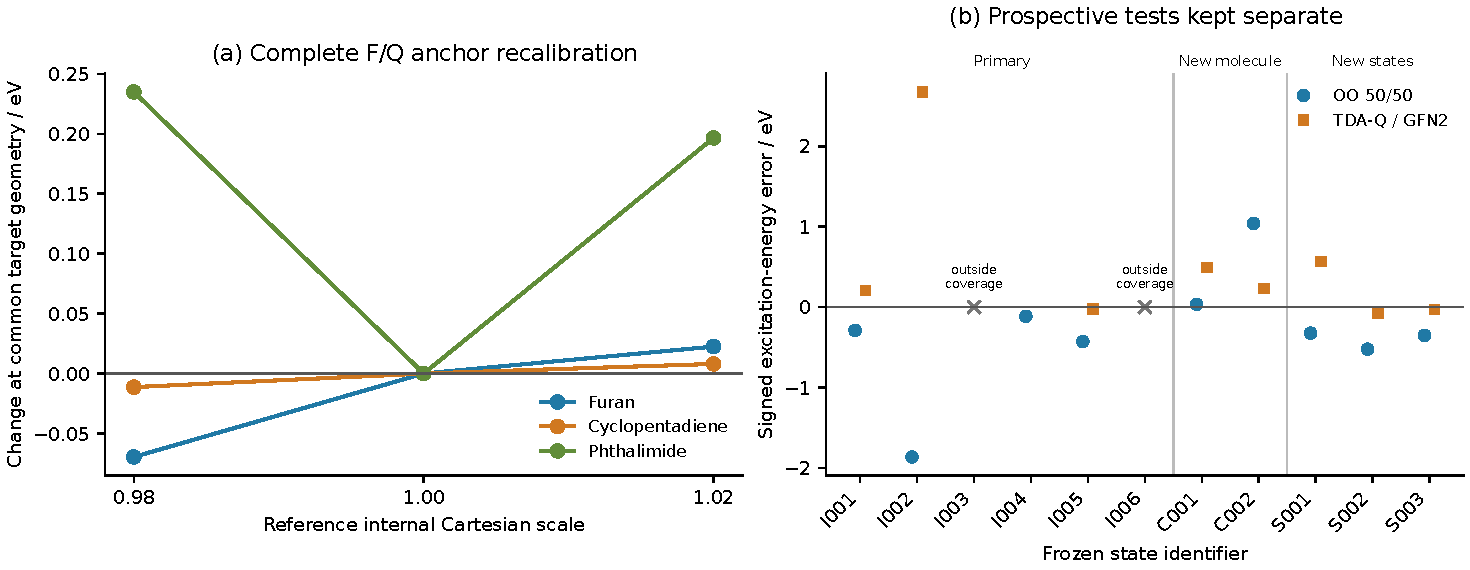
\includegraphics[width=\linewidth]{figures/final_anchor_independent.pdf}
\caption{Final common-geometry anchor test and separately identified prospective cohorts. Crosses indicate inadequate compact-space coverage, not zero error. Both-parent operators are fully recalibrated in panel (a). Signed errors in panel (b) retain partial-double-character and unsafe-reference flags in the accompanying table.}\label{fig:finalvalidation}
\end{figure}

\subsection{Physical curvature and symmetry-breaking descent}
For furan, the symmetric valence A1 stationary structure is compared with the corresponding EOM-CCSD stationary point of Gromov et al.\cite{furan2003} Five bond lengths give a mean absolute difference of 0.0237~\AA, and five angles give $1.55^\circ$. Fifteen in-plane frequencies, matched by symmetry then frequency order, give 188.6~cm$^{-1}$ MAE; a 1474~cm$^{-1}$ B2 discrepancy is retained. Cross-method mode-vector overlaps are unavailable. The model has five negative out-of-plane modes, consistent with treating this structure as a stationary saddle rather than a minimum; the reference also identifies out-of-plane instability. Displaced-gradient checks along the most negative and highest positive modes verify the analytic curvatures. A further bounded nonsymmetric descent preserves lower-energy accepted checkpoints but does not certify a furan minimum.

The analogous cyclopentadiene descent does reach a minimum of the frozen upper A1 surface: the maximum gradient is $2.59\times10^{-5}$~\Eh/bohr and all 27 vibrational frequencies are positive, from 204.8 to 2961.2~cm$^{-1}$. Its total energy is 0.01804~\Eh\ below the symmetric stationary point. A separate central difference of total gradients along its softest vibrational mode agrees with the analytic Hessian action within $1.33\times10^{-10}$~\Eh/bohr$^2$. This is a model minimum, not a correlated-reference validation of that upper-state minimum. Local coherent CSF following is used only for continuous geometry paths; vertical target assignment retains the frozen reference transition. A distorted furan point independently verifies the total energy gradient within $2.46\times10^{-9}$~\Eh/bohr.

\begin{figure}[!htbp]
\centering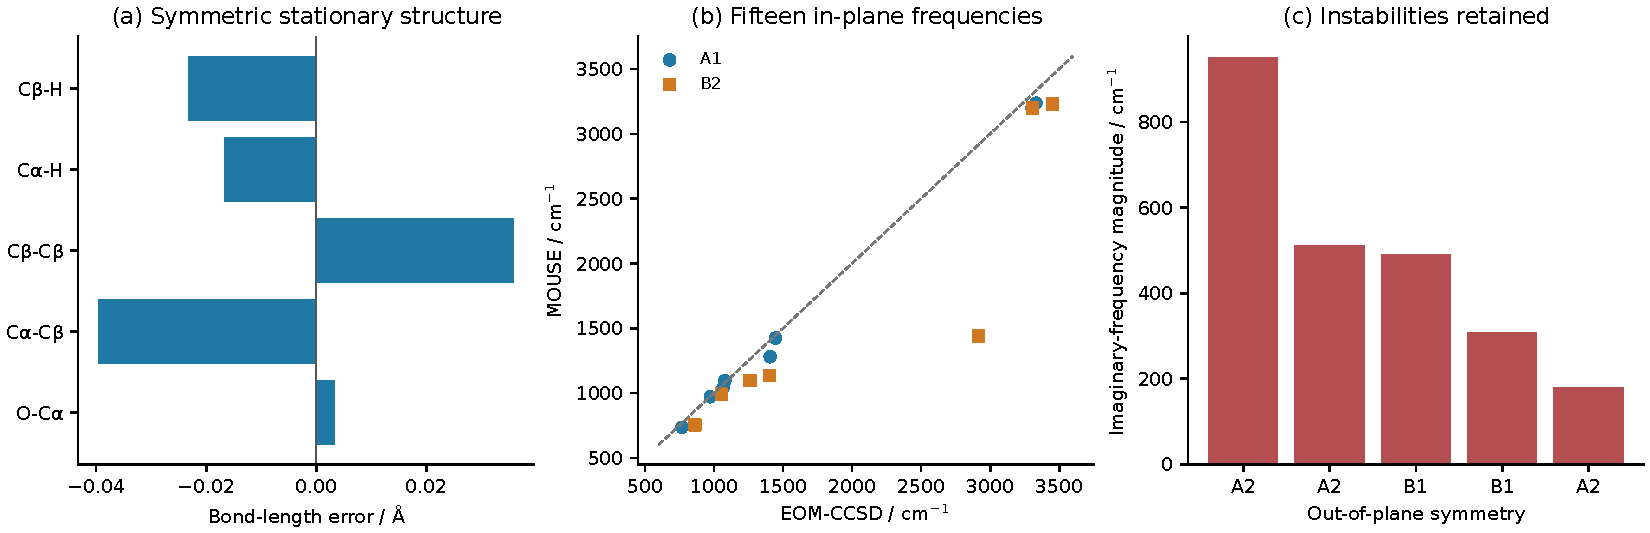
\includegraphics[width=\linewidth]{figures/furan_physical_validation.pdf}
\caption{Furan comparison at the symmetric A1 valence stationary point. EOM-CCSD data are from Tables V and VI of Ref.~\citenum{furan2003}. In-plane mode correspondence uses symmetry and frequency ordering. Imaginary model modes are shown explicitly; no unpublished reference frequencies are assigned to them.}\label{fig:furanphysical}
\end{figure}

The same analytic implementation now completes the full $48\times48$ phthalimide Hessian. Batched response and orbital-block reuse reproduce the first complete calculation, which still rebuilt the duplicate orbital block, within $1.32\times10^{-12}$~\Eh/bohr$^2$. A controlled two-step relaxed-gradient difference has quadratic step convergence and agrees after extrapolation within $4.42\times10^{-7}$~\Eh/bohr$^2$. Translation and nonstationary rotation identities also pass. No finite-difference Hessian enters production.

\subsection{Final cost and preparation accounting}
Six sizes are measured on the dual-socket AMD EPYC 7543 Oracle node (128 logical CPUs) with two threads and an exclusive campaign compute lock. Fresh processes time the prepared energy, energy plus total gradient, energy plus gradient and analytic Hessian, and both-parent all-root singlet TDA on corrected GFN2 orbitals. Three repeats are retained for nitroxyl, acetaldehyde and acetone; a closing budget fixed before larger-case measurements uses one for furan, cyclopentadiene and phthalimide. Model loading and converged-ground setup are outside the property timer; peak RSS covers the whole process. The first three cases use one CSF per parent and the last three two, so this is a practical size/rank benchmark. After exact nuclear-response acceleration, every affected gradient and Hessian timing is remeasured. Unaffected energy-only and TDA measurements are retained, with their execution hashes. External server load and single-repeat large-case variability limit fine timing comparisons.

Across all six measured sizes, the retained prepared OO energy costs more than the complete both-parent TDA evaluation: 0.286--11.478~s versus 0.014--8.731~s. Thus no energy-only speed advantage is observed, even though TDA produces more roots. The intended contribution is the stationary energy surface and its complete analytic nuclear response.

With the contracted response, furan takes 0.851~s for energy plus gradient and 5.104~s including its analytic Hessian; cyclopentadiene takes 1.042 and 7.083~s. Their previous Hessian times were 104.156 and 251.653~s, giving measured reductions by factors of 20.4 and 35.5. Phthalimide now completes energy, gradient and the full $48\times48$ analytic Hessian in 42.224~s, compared with the previous right-censored time of at least 600~s: a reduction exceeding 14.2. Its energy-plus-gradient call takes 9.292~s. The maximum whole-process RSS in the updated benchmark is 1.07~GiB; the earlier phthalimide gradient process reached 9.26~GiB. All six Hessians are completed. The 72-row ledger contains 48 measured completed evaluations and 24 prespecified omitted repeats; earlier measurements and the censored attempt remain archived.

\begin{figure}[!htbp]
\centering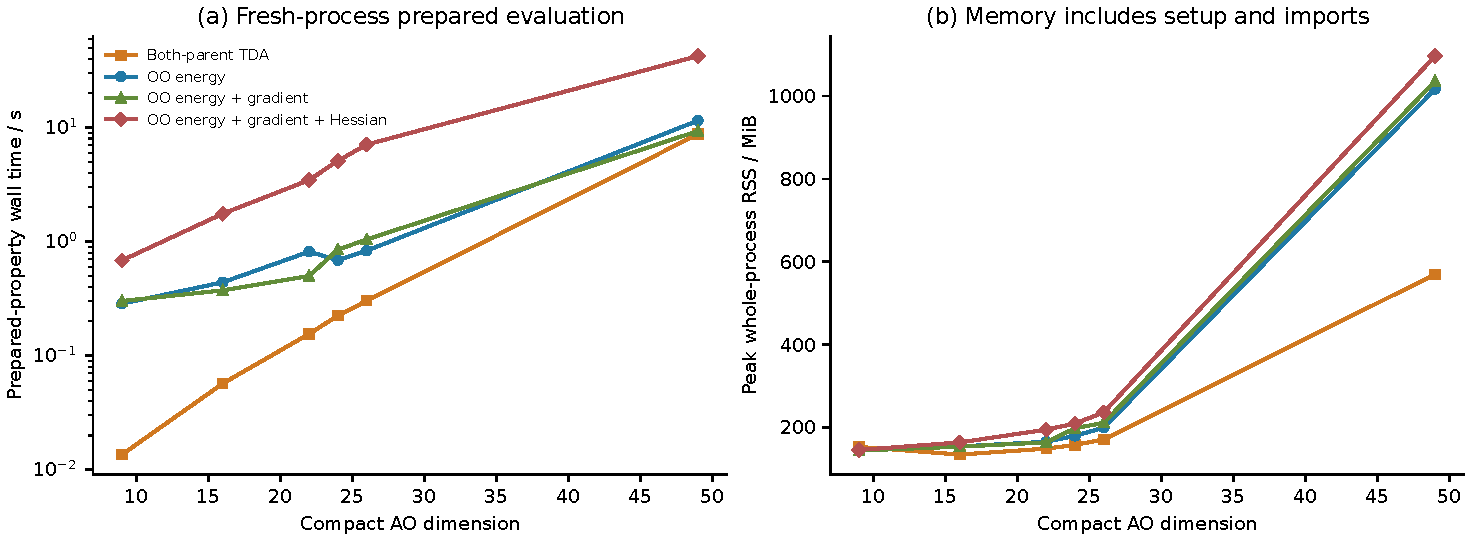
\includegraphics[width=\linewidth]{figures/final_cost_scaling.pdf}
\caption{Prepared-property wall time and whole-process peak RSS after analytic nuclear-response acceleration. Unaffected energy-only and TDA measurements are retained; gradients and Hessians are remeasured. TDA obtains all roots for both parents, whereas OO targets one state. The table records repetitions and ranks. Electronic work from this campaign does not overlap timings; external Oracle load is uncontrolled.}\label{fig:finalcost}
\end{figure}

Preparation is audited rather than assigned zero cost. For the fresh molecular cohort, DFT ground calculations take 0.51--38.13~s, recorded reference-TDA stages 0.88--73.36~s per symmetry, and executed full-response calibrations 1.52--77.17~s. Reference TDA supplies state identity and the active-rank rule: the current preparation therefore requires excited-reference transitions as well as ground-state DFT energies. These stage measurements are from a different cohort and are not missing preparation totals for the six timing molecules. Historical complete cold-preparation totals are unavailable. Consequently, the prepared costs quantify the derivative workload but do not establish an end-to-end advantage over TDA or a fully semiempirical reference preparation.

